\documentclass[output=paper]{langsci/langscibook} 
\ChapterDOI{10.5281/zenodo.3975809}

\author{Geraldine Quartararo \affiliation{Department of Romance Studies and Classics, Stockholm University}} 

\title{Epistemic uses of the \textit{pretérito} \textit{pluscuamperfecto} in La Paz Spanish}
\shorttitlerunninghead{Epistemic uses of PPl in La Paz Spanish}

 

\abstract{This paper explores epistemic-evidential uses of the pluperfect, i.e. \textit{pretérito pluscuamperfecto}, in La Paz Spanish. The \textit{pretérito pluscuamperfecto} displays functions of a reported evidential form, conforming to results from previous studies on Argentinian Spanish (\citealt{Bermudez2008}; \citealt{Speranza2014}) and, furthermore, is used according to a previously unnoticed inferential evidential function. Using theoretical frameworks from \citet{Kockelman2004} and \citet{Bergqvist2018c}, this paper describes the configuration of participant roles and event types implied in the different evidential functions of the \textit{pretérito pluscuamperfecto}.
% \keywords{reported evidentiality, inferential evidentiality, mirativity, event types, participant roles.}
}

\begin{document}
\maketitle

\section{Introduction} 
Romance languages do not possess grammaticalised evidentials and express the evidential domain through verbal inflection. In peninsular Spanish, for instance, the evidential domain is expressed by means of the simple future, the past imperfect, the present conditional and the past conditional. The simple future and the present conditional are used to express inference in the present (\ref{ex:gq1}) and in the past (\ref{ex:gq2}), respectively. 
%\isi{finality} 


\ea \label{ex:gq1}
	\langinfo{Peninsular Spanish}{}{\citealt[317]{Squartini2001}; gloss added}\\
	\gll Ahora \textbf{serán} las cuatro.\\
	now  be.\textsc{fut.3pl} \textsc{art.f.pl} four\\
	\glt ‘It must be (lit. will be) 4 o’clock.’
	\z


	\ea \label{ex:gq2}
	\langinfo{Peninsular Spanish}{}{\citealt[317]{Squartini2001}; gloss added, translation modified}\\
	%\textbf{Serían} las ocho cuando salimos   \\
	\gll \textbf{Serían} las ocho  cuando  salimos.\\
	be.\textsc{con.3pl} \textsc{art.f.pl} eight when go.out-\textsc{pst.1pl}\\
	\glt ‘It was (lit. would be) 8 o’clock when we left.’
	\z


Whereas the imperfect (\ref{ex:gq3}) and the past conditional\footnote{The evidential use of the past conditional is restricted to journalistic or more formal prose \citep[33]{Reyes1996}.}  (\ref{ex:gq4}) are used to express reported evidentiality. 


\ea \label{ex:gq3}
\langinfo{Peninsular Spanish}{}{\citealt[31]{Reyes1996}; gloss added, translation added}\\
	\ea \label{ex:gq3a}
		\gll ¿{Qué tal} sigue Ana?\\
		how follow-textsc{prs.3sg} \textsc{pn}\\
		\glt ‘How is Ana doing?’
	\ex \label{ex:gq3b}
	%\langinfo{}{}{}
	\gll Mejor me parece. No la v-i, porque cuando llegu-é dorm-ía. Pero hab-ía com-ido  algo, y tenía menos fiebre. Esta noche la veía el médico {de nuevo}.\\
    better \textsc{1sg.dat} seem-\textsc{prs.3sg} not \textsc{3sg.f.acc} see-\textsc{pst.1sg} because when arrive-\textsc{pst.1sg} sleep-\textsc{pst.ipfv.3sg} but have-\textsc{pst.ipfv.3sg} eat-\textsc{ptcp} something and have-\textsc{pst.ipfv.3sg} less fever this night \textsc{3sg.f.acc} see.\textsc{pst.ipfv.3sg} the  doctor again\\
	\glt ‘I think she’s better. I did not see her, because when I arrived, she was sleeping. But she had eaten something and had lower fever. Tonight, the doctor is supposedly going to see (lit. saw) her again.’
	\z
\z


\ea \label{ex:gq4}
	\langinfo{Peninsular Spanish}{}{\citealt[317]{Squartini2001}; gloss added, translation modified}\\
	%Según fuentes políticas consultadas por este periódico, Milosevic \textbf{habría} \textbf{aceptado} que la fuerza de interposición en Kosovo esté compuesta por un 30\% de efectivos de la OTAN. (\citealt[317]{Squartini2001}; gloss added, translation modified) \label{ex:gq4}\\
	\gll Según fuente-s políticas consult-ad-as por este periódico, Milosevic \textbf{hab-ría} \textbf{aceptado} que la {fuerza de interposición} en Kosovo est-é compue-sta por un {30\%} de efectivo-s de la OTAN.\\
	according.to source-\textsc{pl} politic-\textsc{pl.f} consult-\textsc{ptcp}-\textsc{pl.f} by this newspaper \textsc{np} have-\textsc{cond.3sg} accept-\textsc{ptcp} that \textsc{art.f.sg} {peacekeeping.force} in Kosovo be-\textsc{subj.1sg} form-\textsc{ptcp.f} by \textsc{art} { } of troop-\textsc{pl} of \textsc{art.f.sg} NATO \\
	\glt ‘According to political sources consulted by this newspaper, Milosevic accepted (lit. would have accepted) the Kosovo peacekeeping force to be composed of 30\% NATO troops.’
\z

With regard to the \textit{pretérito pluscuamperfecto}, Spanish grammars (\citealt{HernandezAlonso1986}, \citealt{Cartagena1999}) describe it as the tense that points out the \textit{consecutio} \textit{temporum} ‘sequence of tenses’ between two past actions: the more recent action is conjugated in imperfect, simple past or present perfect, while the preceding action is in \textit{pretérito} \textit{pluscuamperfecto.}


\ea  \label{ex:gq5}
	\langinfo{Peninsular Spanish}{}{10\_SP\_TASK: 10}\\
	\gll luego mi la mi mujer fue a vend-er lo que \textbf{hab-ía} \textbf{cosech-ado} y yo me fui a sent-ar \\
	then my \textsc{art.f.sg} my woman go.\textsc{pst.3sg} to sell-\textsc{inf} \textsc{3sg.acc} that have-\textsc{ipfv.3sg} harvest-\textsc{ptcp} and I \textsc{1.refl} go.\textsc{pst.1sg} to sit-\textsc{inf}\\
	\glt ‘Then my wife went to sell what she had harvested and I went to sit.’
\z 

Moreover, the \textit{Nueva Gramática de la Lengua Española} (\citealt[542]{RealAcademia2010}) indicates two other uses of the \textit{pretérito pluscuamperfecto}, such as the expression of habitual actions (\ref{ex:gq6}) and politeness (\ref{ex:gq7}).


\ea \label{ex:gq6}
\langinfo{Peninsular Spanish}{}{RAE 2010: 452; gloss added, translation added}\\
\gll A esa hora, los viernes Eugenio \textbf{hab-ía} \textbf{sal-ido} del trabajo.\\
at that hour the friday \textsc{np} have-\textsc{ipfv.3sg} go.out-\textsc{ptcp} from.\textsc{art.sg} work\\
\glt ‘At that time, every Friday, Eugenio went (lit. had gone) out from work.’
\z


\ea  \label{ex:gq7}
	\langinfo{Peninsular Spanish}{}{\citealt[355]{HernandezAlonso1986}; gloss added, translation added}\\
	\gll Hab-ía pens-ado yo ped-ir-le.\\
	have-\textsc{ipfv.3sg} go.out-\textsc{ptcp} I ask-\textsc{inf-3sg.dat}\\
	\glt ‘I was thinking (lit. had thought) to ask him/her.’
\z 


In addition to these normative uses, studies on Latin American Spanish varieties (\citealt{Laprade1981}; \citealt{Mendoza1991};  \citealt{CallisayaApaza2012}; \citealt{Adelaar2004}; \citealt{Speranza2014}; \citealt{Bermudez2008}) have also attested evidential uses of the \textit{pretérito} \textit{pluscuamperfecto} (\ref{ex:gq8}). 


\ea \label{ex:gq8}
	\langinfo{La Paz Spanish}{}{\citealt[224]{Laprade1981}; gloss added, translation modified}\\
	\gll Me \textbf{hab-ía} \textbf{tra-ído} est-a puntabola.\\
	1.\textsc{refl} have-\textsc{ipfv.3sg} bring-\textsc{ptcp} this-\textsc{f} pen\\
	\glt ‘I (accidentally) brought (lit. had brought) this pen with me.’
\z

The specialized literature on the evidential use of the \textit{pretérito} \textit{pluscuamperfecto} in Argentinian Spanish is limited to two studies, i.e. \citet{Bermudez2008} and \citet{Speranza2014}. While questioning the temporal function of the \textit{pretérito} \textit{pluscuamperfecto}, \citet{Bermudez2008} shows four evidential functions of this tense: an ‘external source’, which expresses the perspective of a third party; ‘shared access to information’, marking information also known by the addressee; ‘endophoric source’, marking information that does not come from sensory experience; and finally, ‘mirative’, which marks information that goes against speaker’s expectations. \citet{Speranza2014}, in turn, proposes a sociolinguistic analysis of the uses of the \textit{pretérito} \textit{pluscuamperfecto} and observes a higher number of epistemic-evidential uses in the varieties of Argentinian Spanish that are in contact with languages with grammaticalised evidential-epistemic systems, such as Quechua and Guaraní \citep[26]{Speranza2014}. With respect to the expression of the commitment to the truth of information provided by the \textit{pretérito} \textit{pluscuamperfecto} as evidential-epistemic form, \citet{Bermudez2008} and \citet{Speranza2014} arrive at different conclusions. \citet[217]{Bermudez2008} states that the use of an indirect evidential does not necessarily imply a low commitment to the truth of information: 

\begin{displayquote}
Assigning information to an external source may mean either a weakening, or a strengthening of the reliability of the utterance, this depends on the level of reliability given to the source by the participants involved in the language exchange.\footnote{El asignar una información a una fuente externa puede significar tanto una debilitación como un fortalecimiento de la credibilidad de la afirmación, lo cual depende del nivel de credibilidad concedido a la fuente en cuestión por los participantes del intercambio lingüístico.}	
\end{displayquote}

Whereas \citet[111]{Speranza2014} states more precisely that the use of the \textit{pretérito} \textit{pluscuamperfecto} implies the speaker’s low degree of commitment to the truth of the information provided. 

\begin{displayquote}
The appearance of the PPl (\textit{pretérito} \textit{pluscuamperfecto}) is related to utterances where there is the possibility of greater ambiguity in the attribution of what is mentioned […] the sender, then, expresses a lower degree of reliability by selecting a subordinate tense.\footnote{La aparición del PPl se vincula a emisiones en las que existe la posibilidad de mayor ambigüedad en la atribución de los dichos […] El enunciador, entonces, expresa su menor grado de confiabilidad a través de la selección del tiempo verbal dependiente.}	
\end{displayquote}

I am not aware of a separate study focusing on the epistemic-evidential function of the \textit{pretérito pluscuamperfecto} in Bolivian and Peruvian Spanish, even though this use has been noted in the literature (\citealt[222--225]{Laprade1981}; \citealt[196--203]{Mendoza1991}; \citealt[306--308]{CallisayaApaza2012}; \citealt{Adelaar2004}). \citet[223]{Laprade1981} notices that in La Paz Spanish the \textit{pretérito pluscuamperfecto} can have mirative function or indicate absence of direct knowledge. Along this line, \citet[199]{Mendoza1991} adds a further observation based on phonology, arguing that whenever the \textit{pretérito pluscuamperfecto} has evidential-epistemic function in La Paz Spanish, the auxiliary verb \textit{haber} ‘to have’ shows an accent shifting from \textit{había} to \textit{habiá}. Finally, \citet[307]{CallisayaApaza2012} states that epistemic-evidential uses of the \textit{pretérito pluscuamperfecto} are also found in other regions of Bolivia, although the author does not specify which ones. The contributions of the present study are three-fold. First, it details the epistemic-evidential uses of the \textit{pretérito pluscuamperfecto} in La Paz Spanish. As already mentioned, the use of the \textit{pretérito pluscuamperfecto} as an indirect evidential form has been already described for Argentinian Spanish (\citealt{Speranza2014}; \citealt{Bermudez2008}), but its use in other varieties of Latin American Spanish and, specifically, in Bolivian Spanish has not been accounted for. The second contribution consists of further data that highlights the pragmatic functions of the form in interaction. It is argued that, in its evidential function, the \textit{pretérito pluscuamperfecto} signals the distancing of the speaker from the propositional content of the utterance. Such a distancing, however, is not necessarily related to a low degree of commitment to the truth of the information and, in this regard, the evidential uses of this tense, i.e. inferential or reported, display different outcomes. The third contribution is to give better insights on the configuration of the pragmatic features involved in the use of \textit{pretérito pluscuamperfecto} as evidential form. Following the theoretical framework proposed by \citet{Kockelman2004} and \citet{Bergqvist2018c}, the pragmatic features – such as event types and participant roles – involved in the different evidential functions of the form as well as their distribution are discussed. The first-hand data used in the study were collected in La Paz, Bolivia during 2014 and 2015.

In the remainder of the paper, I will refer to the \textit{pretérito pluscuamperfecto} by the acronym PPl (cf. \citealt{Speranza2014})\footnote{This paper is based on chapter 10 of my PhD thesis \citep{Quartararo2017}.}.


\section{Evidentials, epistemic modality, participant roles and event types}\label{s:gq2}

\citet[3]{Aikhenvald2004} argues that the core meaning of evidentiality is the expression of the source of information, but she notes epistemic extensions for both reported \citep[180]{Aikhenvald2004} and inferential evidential markers \citep[176]{Aikhenvald2004}. Such extensions are usually related to the expression of the speaker’s degree of commitment to the truth of the information, i.e. epistemic modality, and are attested in languages in which the two domains, i.e. evidentiality and epistemic modality, are expressed by the same forms (\citealt[354]{Plungian2001}, cf. Romance languages). The overlap between the two domains is visible in how indirect evidentials may indicate both the speaker’s direct contact with the results of an event, and the lack of such results. This is the case of inferring evidentiality\footnote{Through the term “inferring” Willett indicates both inference, in Willett’s terms “results”, and assumption, in Willett’s terms “reasoning”.} \citep[57]{Willett1988}, as in the use of the Italian future tense in (\ref{ex:gq9}), and reported evidentiality \citep[57]{Willett1988}, as in the use of the Italian conditional mood in (\ref{ex:gq10}). In both cases, the speaker may express different degrees of reliability regarding the verisimilitude of the state of affairs due to the lack of direct evidence.


\ea \label{ex:gq9}
	\langinfo{Italian}{}{\citealt[923]{Squartini2008}; gloss added, translation modified}\\
	\gll [Suon-ano alla porta]. \textbf{Sarà} il postino.\\
	ring-\textsc{prs.3pl} to.\textsc{art.sg} door be.\textsc{fut.3sg} the postman\\
	\glt ‘[The bell rings] It must be (lit. will be) the postman.’
\z


\ea \label{ex:gq10}
	\langinfo{Italian}{}{\citealt[311]{Squartini2001}; gloss added}\\
	\gll Secondo Luca, ieri il treno \textbf{sarebbe} \textbf{part-ito} alle 5.\\
	according.to \textsc{pn} yesterday the train be.\textsc{cond.3sg} leave-\textsc{ptcp} to.\textsc{art.pl} 5\\
	\glt ‘According to Luca the train left (lit. would have left) at 5 yesterday.’
\z

In recent years, some studies on the pragmatic properties of evidentials (\citealt{Curnow2002b}, \citeyear{Curnow2003}; \citealt{Clift2006}; \citealt{Faller2006};  \citealt{Hengeveld2015}) have significantly contributed to the description of semantic extensions acquired by evidentials in specific communicative contexts. Such studies have also provided better insights into the pragmatic features involved in the use of evidentials. \citet[172]{Hanks2012} summarizes three pragmatic dimensions that affect the use of evidentials: \textit{source of knowledge}, i.e. the source on which the information rests; \textit{source of statement}, i.e. the source of the utterance provided; and \textit{expressivity/interaction force}, i.e. the “subjective relation between the speaker and some element of the utterance context” \citep[174]{Hanks2012}. The first and third pragmatic dimensions (i.e. source of knowledge and expressivity) have been detailed in studies on evidentials, both from a typological perspective (\citealt{Willett1988}; \citealt{DeLancey1997}; \citealt{Plungian2001}; \citealt{Aikhenvald2004}) and in language specific descriptions (\citealt{Curnow2002b}, \citeyear{Curnow2003}; \citealt{Clift2006}; \citealt{Babel2009}), but the second pragmatic dimension, \textit{source of statement}, has received less attention in the literature. According to \citet[174]{Hanks2012}, two kinds of possible pragmatic effects belong to the \textit{source of statement}, i.e. the \textit{discourse modality} and the \textit{participant roles}. \textit{Discourse modality} refers to the perspective that speakers adopt in shaping their utterance. In this respect, \citet{Nuckolls2012} demonstrates that, in Pastaza Quichua, the use of different evidential markers in conversational context does not necessarily indicate the access to information, but it can also specify the perspective adopted by speakers towards the information.


\ea \label{ex:gq11}
\langinfo{Pastaza Quichua}{Quechua languages, Ecuador y Perú}{\citealt[231]{Nuckolls2012}; gloss modified}\\
	\ea \label{ex:gq11a}
		\gll Ñuka-ta ña kai ruya-ta rikwi-i chi sʰapi-\textbf{mi} siri-u-n.\\
	I-\textsc{acc} now this tree-\textsc{acc} look-\textsc{imp} that base-\textsc{ev} lie-\textsc{dur-3sg}\\
	\glt ‘Look at me (up in) this tree! It’s lying right at that base!’ (Context: The speaking self of the narrative event (-mi sⁿ) where Luisa becomes the voice of Tito talking to his friend)
	\ex \label{ex:gq11b}
	\gll Ni-sha-\textbf{shi} kapari-ni.\\
	say-\textsc{cor-evd} shout-\textsc{1sg}\\
	\glt ‘Saying (according to my husband) I shout.’ (Context: The voice of the other (-shi), where Luisa specifies the perspective of Tito who was asserting something to her)
	\z
\z

In examples (\ref{ex:gq11a}) and (\ref{ex:gq11b}), the use of two markers, i.e. the direct evidential -\textit{mi} and the reported evidential -\textit{shi}, does not signal a difference in the way Luisa has gained access to information. Since in both cases Luisa heard Tito’s words, it rather points out the two different perspectives from which Luisa is providing the information. In (\ref{ex:gq11a}), by using the evidential marker -\textit{mi,} she provides information from Tito’s perspective who \textit{de facto} pronounced the words that she is reporting. In (\ref{ex:gq11b}), on the other hand, by using the evidential marker -\textit{shi,} Luisa maintains her perspective and distances herself from Tito’s words.

The change of perspective implied by the use of different evidentials, as shown for Pastaza Quichua, is essential to clarify the relevance of the second class of pragmatic effects established by \citet{Hanks2012}, i.e. \textit{participant roles}. Drawing on \citegen{Goffman1981} classification, speakers can be said to occupy three roles, namely, \textit{principal}, \textit{author} and \textit{animator}. The \textit{principal} is the one responsible for the utterance, i.e. the last person who committed to the information provided. The \textit{author} is the person who has chosen the words of the utterance in the narrated world \citep{Goffman1981}, i.e. who has pronounced it for the first time. Finally, the \textit{animator} is the person who physically produces the utterance. The three roles generally overlap within the same speaker, e.g. in the sentence “I am fine”, the speaker is \textit{principal} since s/he is taking responsibility for his/her own emotional and health status, as well as \textit{author} and \textit{animator} since s/he chooses the words of the statement and physically utters them. 

Further elements of the description of the pragmatic features involved in the use of evidentials are provided by \citet{Kockelman2004} and \citet{Bergqvist2018c}. \citet{Kockelman2004} proposes an implementation of \citegen{Jakobson1957} classification of event types by adding a \textit{commitment event}, and by expanding the \textit{narrated speech event} to apply to all evidential notions, calling it \textit{source event}. The resulting set of event types is composed by the \textit{speech event}, the \textit{narrated event}, the \textit{source event} and the \textit{commitment event}. The \textit{speech event} corresponds to the world in which the utterance is made. The \textit{source event} corresponds to the “spoken-about world in which speaking occurs” \citep[128]{Kockelman2004}, and may be distinguished according to the type of contact that a speaker has with a source \citep[143]{Kockelman2004}. The \textit{narrated event} indicates the world described in the utterance. Finally, the \textit{commitment event} is the world where the speaker commits to the truth of the proposition expressed \citep[127]{Kockelman2004}. In addition to this proposal, \citet{Kockelman2004} also establishes a correlation between \citegen{Goffman1981} participant roles, i.e. \textit{animator}, \textit{author} and \textit{principal}, and the new set of event types, i.e. the \textit{speech event}, the \textit{narrated event} and the \textit{commitment event}. Within this framework, \citet{Bergqvist2018c} formulates another relation that connects \textit{source event} \citep[128]{Kockelman2004} with a new participant role defined as \textit{cognizer} \citep[22]{Bergqvist2018c}, i.e. the person who perceives the event. This set of correspondences is illustrated in \ref{tab:fig:gq1}.

%figure 1
\begin{table}
\begin{tabularx}{.75\textwidth}{CL{1cm}C}
\lsptoprule
Event Type &  & Speaker Role \\
\midrule
speech event & \Leftrightarrow & animator \\
source event & \Leftrightarrow & cognizer \\
narrated event & \Leftrightarrow & author \\
commitment event & \Leftrightarrow & principal \\
\lspbottomrule
\end{tabularx}
\caption{Correspondence between event types and participant roles}
\label{tab:fig:gq1}
\end{table}


If one takes the model of correspondences shown in \ref{tab:fig:gq1}, and applies this to Example (\ref{ex:gq11}), above, it becomes possible to provide an analysis of the pragmatic features relevant to the use of evidentials. In (\ref{ex:gq11a}), Luisa produces the utterance as if Tito was pronouncing it. This strategy results in two series of consequences in the configuration of the correlation between event types and participant roles: first, by reproducing Tito’s voice, Luisa creates an artificial overlap between the participant roles of the two speakers, playing simultaneously the \textit{animator} (Luisa is indeed the last who pronounced the utterance), the \textit{author} (Tito has chosen the words of the information), the \textit{cognizer} (Tito witnessed the event) and the \textit{principal} (Tito committed to the truth of his statement); second, by impersonating Tito’s voice, Luisa fictitiously matches the world in which she is pronouncing the utterance with the world in which Tito pronounced the utterance, i.e. the \textit{speech event} overlaps with the \textit{source event}, since they fictitiously occur in the same world. Given the use of the direct evidential -\textit{mi,} the \textit{commitment event} coincides with the \textit{source event}. Finally, considering that the \textit{narrated event} does not make any reference to the world in which the \textit{speech event} occurs (e.g. in “I promise”), it will be kept separate from the others. In (\ref{ex:gq11b}), the configuration of event types and participant roles is different. By using the reported evidential -\textit{shi}, instead, Luisa specifies the separation between the \textit{speech event} and the \textit{source event}, the \textit{narrated event} is kept distinguished from the previous two event types and, finally, the configuration of the \textit{commitment event}, as for the correlated participant role, cannot be established. 

\section{Material, participants and method}\label{s:gq3}

Thirty Spanish-Aymara bilingual speakers participated in the study (17 males and 13 females, age range: 18--64). All participants first learned Aymara and then acquired Spanish during their childhood. The L2 proficiency in the standard variety of La Paz Spanish varied among the speakers depending on age and level of education. About 60\% of the speakers had university level education, 26,6\% had secondary education and 13,4\% had primary education. 

The data was collected mainly in La Paz and El Alto (Bolivia). The corpus consists of fully transcribed recordings lasting 8 hours and 24 minutes in total. The transcription convention employed (\citealt{Briz2000}) has also been used for the transcription of colloquial Spanish corpora and allows for a faithful representation of speech. 

The corpus is divided into three parts: the first and largest part consists of the recordings of the “Family Problems Picture Task” (\citealt{SanRoqueetal2012}), the second part consists of five recordings of the task “The Pear Story” \citep{Chafe1980}, and the third part consists of four recordings of personal narratives.

The “Family Problems Picture Task” (FPPT) was created to activate the use of cognitive categories such as evidentiality and mirativity (\citealt[140]{SanRoqueetal2012}). Its two-fold nature of problem-solving and interactive task allows the activation of inferential processes and, therefore, supports the analysis of the use of evidentials in interactive settings. The task consists of 16 pictures in black and white that follow a defined order. The temporal sequence and content of the pictures are not always clear. Inferential processes are required to understand the order and development of the story. 

The FPPT was developed in five steps: in the first step, speakers were asked to describe five of the sixteen pictures randomly selected by the fieldworker; in the second step, speakers ordered all the pictures according to the story that they believed it was represented; in the third step, one of the two participants in the first two steps was asked to describe the story built in the first person singular; in the fourth step, the other participant was asked to tell the story in the third singular person to a third person who did not participate in the task until then; finally, during the fifth step, the third participant was asked to tell the story s/he had been told. In order to facilitate data analysis, the internal organization of the transcriptions follows the same structure of the FPPT, i.e. each transcription is divided into five parts. 

\section{The epistemic-evidential functions of the PPl}\label{s:gq4}

The corpus features 78 tokens of the PPl. The analysis reveals that in most of the cases, 68\%, the PPl is used according to its temporal function (see example \ref{ex:gq5}), i.e. it indicates the temporal relation between two past actions; nevertheless, in a significant number of cases, 32\%, the PPl seems to operate as an epistemic-evidential form, i.e. it specifies the epistemic relation between the speaker and the event. When the PPl is used as an epistemic-evidential form, it may display inferential evidence, reported evidence or mirativity. As an inferential evidential, the PPl signals inference based on observable evidence (13 cases). As a reported evidential, it signals second-hand report, i.e. the speaker has directly heard the words of someone else (9 cases). Finally, as mirative form, it indicates surprise (2 cases). \tabref{tab:gq1} summarizes this.

\begin{table}
\centering
\begin{tabularx}{.75\textwidth}{Xr}
\lsptoprule
\textbf{Function} & \textbf{№ of cases}\\
\midrule
Temporal function & 54\\
Mirative function & 2\\
Inferring results function & 13\\
Reported second-hand function & 9\\
\hline
Total & 78\\
\lspbottomrule
\end{tabularx}
\caption{Function of the PPl in the data}\label{tab:gq1} 
\end{table}

In the corpus, over 90\% of the occurrences of the PPl (72 cases out of 78) comes from the transcriptions of the FPPT; the remaining cases come from the transcriptions of the personal narratives. By analyzing the distribution of these 72 cases among the steps of the FPPT, it turns out that the PPl appears 8 times during the first step, 5 times during the second step, 24 times during the third step, 22 times during the fourth step, and 13 times during the fifth step. By further narrowing down this analysis to the cases in which the PPl seems to operate as an epistemic-evidential forms, it is notable that all cases of PPl with evidential-epistemic functions occur within the transcriptions of the FPPT. Secondly, no case of inferences based on observable results occurs in the third (i.e. narrative in the first person) and the fifth step of the task (i.e. report of the story to a third participant). Lastly, the largest number of cases of the second-hand reported function appears in the fifth step. This distribution is presented in \tabref{tab:gq2}. 

\begin{table}
\begin{tabularx}{\textwidth}{lYYrr}
\lsptoprule
 \textbf{FPPT} & \textbf{\mbox{Inferring results} evidence} & \textbf{Second-hand reported evidence} & \textbf{Mirativity} & \textbf{Total}\\
\midrule
Step I & 2 & 1 & 2 & 5\\
Step II & 3 & {-} & {-} & 3\\
Step III & {-} & 1 & {-} & 1\\
Step IV & 8 & {-} & {-} & 8\\
Step V & {-} & 7 & {-} & 7\\
\hline
\textbf{Total} & 13 & 9 & 2 & 24\\
\lspbottomrule
\end{tabularx}
\caption{Evidential functions of the PPl (columns) for the steps of the FPPT (rows)}\label{tab:gq2}
\end{table}


\subsection{Mirative or inferential function?}\label{s:gq4-1}

The debate on the relation between evidentiality and mirativity is still an open one. On the one hand, some scholars discuss the nature of the relation between the two domains: \citet{DeLancey1997} and \citet{Aikhenvald2004} consider them as separate, while \citet{Lazard1999} and \citet{Haan2012} consider them to be related. On the other hand, recent studies \citep{Hill2012} entirely reject the description of mirativity as an independent category, arguing that direct evidence (“sensory evidence” in Hill’s terms) is an adequate category to account for most of the markers described as miratives in the literature. 

Taking into account cases in which the use of the PPl is related to the expression of a direct, visual contact with the discourse object, the data shows three situations: (i) the PPl can simultaneously signal both an inferential and a mirative function (example \ref{ex:gq12}), (ii) the PPl can signal only inference (example \ref{ex:gq13}) and, (iii) the PPl can signal only mirativity (example \ref{ex:gq14}).

In a few cases, it is not possible to establish a clear distinction, or a hierarchy between the inferential \citep{Willett1988} and the mirative function of the PPl; the two functions, indeed, seem to co-exist and overlap within the same form, i.e. the PPl [cf. \ref{ex:gq12}]. 

\ea \label{ex:gq12}
\langinfo{La Paz Spanish}{}{5\_SP\_TASK: 6}\\
	\ea \label{ex:gq12a}
	\gll El mismo es.\\
	the same be.\textsc{prs.3sg}\\
	\glt ‘It is the same.’
	\ex \label{ex:gq12b}
	\gll  El mismo con su mujer.\\
	the same with \textsc{3.pos} woman\\
	\glt ‘The same with his wife.’
	\ex  \label{ex:gq12c}
	\gll ...\\
	{...}\\
	\glt ...
	\ex \label{ex:gq12d}
	\gll \textbf{aaaa} \textbf{hab-ía} \textbf{sido} agricultor el cuate\\
	\textsc{interj} have-\textsc{pst.ipfv.3sg} be.\textsc{ptcp} farmer the guy\\
	\glt ‘Aaaa he is (lit. had been) a farmer, the guy’
	\ex \label{ex:gq12e}
	\gll est-án cosech-ando no\\
	be-\textsc{prs.3pl} harvest-\textsc{ger} no\\
	\glt ‘They are harvesting, aren’t they?’
	\ex \label{ex:gq12f}
	\gll est-án cosech-ando sí el  campo es\\
	be-\textsc{prs.3pl} harvest-\textsc{ger} yes the countryside be.\textsc{prs.3sg}\\
	\glt ‘They are harvesting, yes, it is in the countryside’
	\z
\z

% figure 2 
\begin{figure}[ht]
\centering
\begin{subfigure}{0.4\textwidth}
\centering
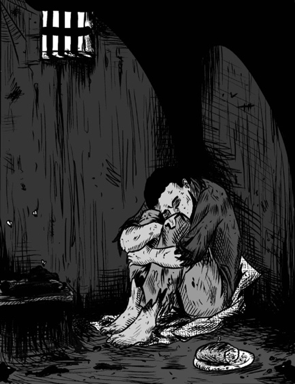
\includegraphics[width=.5\linewidth]{figures/quartaro-fig1_3.png}  
\caption{ } %picture 3
\end{subfigure}
\begin{subfigure}{0.4\textwidth}
\centering
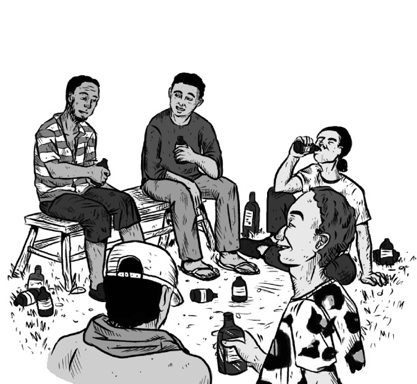
\includegraphics[width=.5\linewidth]{figures/quartaro-fig2_12.png}
\caption{ } %picture 12
\end{subfigure}
\bigskip 
\begin{subfigure}{0.4\textwidth}
\centering
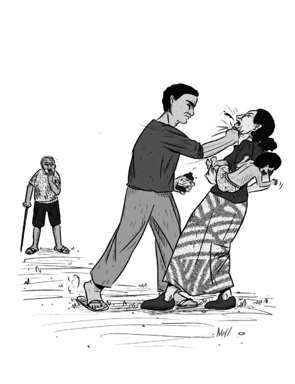
\includegraphics[width=.5\linewidth]{figures/quartaro-fig3_5.png}
\caption{ } %picture 5
\end{subfigure}
\begin{subfigure}{0.4\textwidth}
\centering
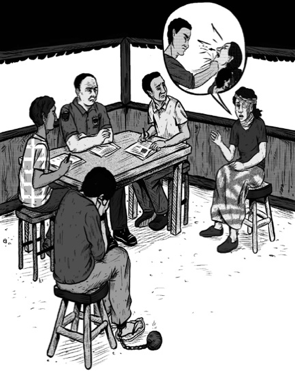
\includegraphics[width=.5\linewidth]{figures/quartaro-fig4_7.png}
\caption{ } %picture 7 
\end{subfigure}
\begin{subfigure}{0.4\textwidth}
\centering
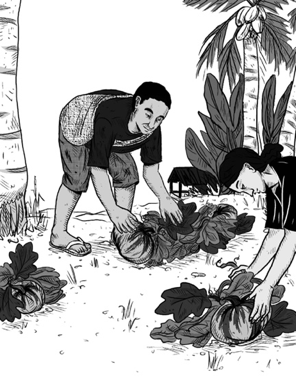
\includegraphics[width=.5\linewidth]{figures/quartaro-fig5_8.png}
\caption{ } %picture 8
\end{subfigure}
\caption{Pictures used during the first step of FPPT}
\label{fig:gq2}
\end{figure}

In (\ref{ex:gq12}), the speakers are describing picture (e) in \figref{fig:gq2}, which is the fifth image shown to participants during the first step of the FPPT, showing a man and a woman that are picking pumpkins in a garden. The remaining four pictures, previously shown to the participants during this stage of the task, depict the man in a cell (picture \ref{fig:gq2}a), drinking alcohol (picture \ref{fig:gq2}b), hitting his wife (picture \ref{fig:gq2}c), and standing in a courtroom (picture \ref{fig:gq2}d).


From observing the first four pictures, speakers are not expected to be able to guess the man’s profession. Picture \ref{fig:gq2}e appears to present new and partly surprising information, indicated by rising intonation and the interjection “aaaa” (see Example \ref{ex:gq12}, above). Although a mirative function is implied by this specific use of the PPl, it is clear that an ongoing inferential process is at the foundation of the information provided. There is no doubt, that in (\ref{ex:gq12}) the sentence where the PPl occurs is an inference, given the fact that no pictures in the task clearly show that the man’s profession is farming. A further instance of this evidential function of the PPl is found in (\ref{ex:gq13}). 

% %TODO space between unglossed examples?!
\ea \label{ex:gq13}
\langinfo{La Paz Spanish}{}{3\_SP\_TASK: 11--12}\\
	\ea \label{ex:gq13a}
	\gll aquí qué est-á hac-iendo este señor ya le empiez-a a cont-ar ha  deb-ido est-ar lejos trabaj-ando este señor {tal vez} le empiez-a a cont-ar su señora a su hijo todo el suceso como hac-ía como trabaj-aba no\\
	here what be-\textsc{prs.3sg} do-\textsc{ger} this man already \textsc{3sg.dat} start.\textsc{prs.3sg} to tell-\textsc{inf} have.\textsc{prs.3sg} must-\textsc{ptcp} be-\textsc{inf} far.away work-\textsc{ger} this man maybe \textsc{3sg.dat} start-\textsc{prs.3sg} to tell-\textsc{inf} \textsc{3.pos} wife to \textsc{3.pos} son all the happening how do-\textsc{pst.ipfv.3sg} how work-\textsc{pst.ipfv.3sg} no\\
	\glt ‘Here, what is this man doing? Aaa now he starts to tell. He must be far away, this man, maybe. He starts to tell his wife and his son everything happened. How he did, how he worked, no?’
	\ex \label{ex:gq13b}
	\gll y su esposa escuch-a.\\
	and \textsc{3.pos} wife listen-\textsc{prs.3sg}\\
 	\glt ‘And his wife listens’
	\ex \label{ex:gq13c}
	\gll y acá empiez-a a trabaj-ar deb-e ser al día siguiente o más tarde no ambos trabaj-aban recog-en su-s zapallo-s\\
	and here start-\textsc{prs.3sg} to work-\textsc{inf} must-\textsc{prs.3sg} be.\textsc{inf} to.\textsc{art.sg} day next or more late no both work-\textsc{pst.ipfv.3pl} pick-\textsc{prs.3pl} \textsc{3pos-pl} pumpkin-\textsc{pl}\\
 	\glt ‘And here they start to work, it must be the day after or later, no? both work, they are picking pumpkins’ 
	\ex \label{ex:gq13d}
	\gll zapallo-s\\
	pumpkin-\textsc{pl}\\
	\glt ‘Pumpkins’ 
	\ex \label{ex:gq13e}
	\gll {o sea} est-as persona-s son agricultor-es\\
	that.is.\textsc{interj} this-\textsc{f.pl} person-\textsc{pl} be.\textsc{prs.3pl} farmer-\textsc{pl}\\
	\glt ‘That is, these people are farmers’
	\ex \label{ex:gq13f}
	\gll  aquí est-án llev-ando zapallo-s\\
	here be-\textsc{prs.3pl} carry-\textsc{ger} pumpkin-\textsc{pl}\\
	\glt ‘Here, they are carrying pumpkins’
	\ex \label{ex:gq13g}
	\gll  es-os zapallo-s que han recog-ido llev-an a vend-er a la feria allí es con su hij-ito es más pequeño\\
	that-\textsc{m.pl} pumpkin-\textsc{pl} that have.\textsc{3pl} pick-\textsc{ptcp} carry-\textsc{prs.3pl} to sell-\textsc{inf} to \textsc{art.f.sg} market there be.\textsc{prs.3sg} with \textsc{3.pos} son-\textsc{dim} be.\textsc{prs.3sg} more small\\
	\glt ‘Those pumpkins that they picked. They are carrying to the market. There he is with his little son, he is younger’ (glossed)
	\ex \label{ex:gq13h}
	\gll más pequeñ-ito Yola\\
	more small-\textsc{dim} Yola.\textsc{pn}\\
	\glt ‘Younger Yola’ (glossed)
	\ex \label{ex:gq13i}
	\gll \textbf{hab-ía} \textbf{ten-ido} dos hijo-s.\\ 
	have-\textsc{pst.ipfv.3sg} have-\textsc{ptcp} two child-\textsc{pl}\\
	\glt ‘He must have (lit. had had) two children’ (glossed)
	\ex \label{ex:gq13j}
	\gll dos hijo-s aquí est-á\\
	two child-\textsc{pl} here be-\textsc{prs.3sg}\\
	\glt ‘two children? Here it is’ (glossed)
	\ex \label{ex:gq13k}
	\gll ya aquí\\
	\textsc{interj} here\\
	\glt ‘Yes, here’ (glossed)
	\z
\z

Example (\ref{ex:gq13}) is an extract from the second stage of the FPPT. Here, the PPl is the main verb of the utterance \textit{había tenido dos hijos} ‘s/he must have had two children’. The speakers placed the pictures of the story in the order shown in \figref{fig:gq3}. %13, 8 and 6.

% figure 3
\begin{figure}
    \centering
    \begin{subfigure}[t]{.4\linewidth}
    \centering
    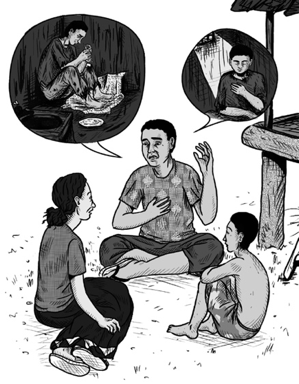
\includegraphics[width=.5\linewidth]{figures/quartaro-fig6_13.png}
    \caption{ } %picture 13
    \end{subfigure}
    \begin{subfigure}[t]{.4\linewidth}
    \centering
     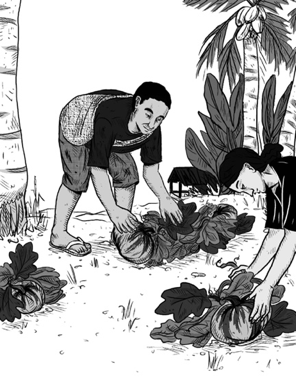
\includegraphics[width=.5\linewidth]{figures/quartaro-fig5_8.png}
     \caption{  }%picture 8
    \end{subfigure}
    \begin{subfigure}[t]{.4\linewidth}
      \centering
    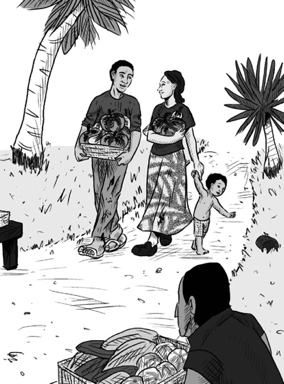
\includegraphics[width=.5\linewidth]{figures/quartaro-fig7_6.png}
    \caption{ } %picture 6
    \end{subfigure}
    \caption{Pictures used during the second step of FPPT} \label{fig:gq3}
\end{figure}

In picture \ref{fig:gq3}a, a man sits talking to a woman and a boy. In picture \ref{fig:gq3}b, the same man is picking pumpkins in a garden with a woman. Finally, in picture \ref{fig:gq3}c, the man, the woman and a small child are walking together down a road, carrying two baskets full of pumpkins. After putting in order the three pictures, the speakers imagine that the actions depicted in them are performed in a few days, \textit{debe} \textit{ser} \textit{al} \textit{día} \textit{siguiente} \textit{o} \textit{más} \textit{tarde} ‘it must be the day after or later’. Furthermore, by comparing picture \ref{fig:gq3}a to picture \ref{fig:gq3}c, they cannot help but notice the presence of two children with different ages. This visually available evidence produces the inference made by B that the couple has two children (\textit{había} \textit{tenido} \textit{dos} \textit{hijos}). 

If in the previous cases (example \ref{ex:gq12} and \ref{ex:gq13}) the use of the PPl is related to an ongoing inferential process, in two cases, the PPl seems to operate exclusively as a mirative form indicating the surprise of the speaker with respect to something drawn in the pictures.

\ea \label{ex:gq14}
\langinfo{La Paz Spanish}{}{5\_SP\_TASK: 5}\\
	\gll uuu qué pas-a aquí a su mujer le \textbf{hab-ía} \textbf{peg-ado} ese maricón\\
	\textsc{interj} what happen-\textsc{prs.3sg} here to his wife \textsc{3sg.dat} have-\textsc{pst.ipfv.3sg} hit-\textsc{ptcp} that wimp\\
	\glt ‘Uuu, What’s happening here? That wimp has hit (lit. had hit) his wife!’
\z

In Example (\ref{ex:gq14}), taken from the first stage of the task, the speaker is describing what is drawn in picture \ref{fig:gq2}c. The use of the PPl, in this case, does not signal an inference, nor is it possible to consider this use of the form as related to other documented uses of the PPl in Spanish such as the expression of \textit{consecutio} \textit{temporum}, politeness or habitual aspect. Given the linguistic elements that co-occur with the PPl in Example (\ref{ex:gq14}), i.e. the interjection “uuu”, the appellative \textit{ese} \textit{maricón} ‘that wimp’, and the exclamatory form of the utterance, the function of the PPl aligns better with the speaker’s (negative) surprise of the man hitting the woman in the picture. This use of the PPl could therefore be said to be an instance of the mirative function, also conforming to mirative uses of this tense as noticed for Argentinian Spanish \citep{Bermudez2008}.

\subsection{Secondhand reported evidential function}\label{s:gq4-2}

As a reported evidential, the PPl always signals second-hand reports, meaning that the speaker reports something that s/he has heard directly from the \textit{author} of the utterance.

According to Spanish grammars \citep{Maldona1999}, indirect speech is constructed through a conjugated reporting verb followed by the complementizer \textit{que} ‘that’ and a subordinate clause, whose verb is conjugated according to specific tense agreement rules. If the reporting verb is in the present tense, then the verb of the subordinate clause will also be in the present tense, the simple past/present perfect/imperfect, or in the future tense. In the subordinate clause, the use of one tense rather than another depends on the original tense of the verb of the reported utterance.

\ea La Paz Spanish (2\_SP\_TASK: 20), speaker A \label{ex:gq15}\\
%\langinfo{La Paz Spanish}{}{2\_SP\_TASK: 20}\\
	\gll uno de su-s familiar-es lo \textbf{ha} \textbf{llev-ado} prenda-s\\
	one of \textsc{3.pos}-\textsc{pl} relative-\textsc{pl} \textsc{3sg.acc} have-\textsc{prs.3sg} take-\textsc{ptcp} cloth-\textsc{pl}\\
	\glt ‘one of his relatives has brought him clothes’
\z	

\ea La Paz Spanish (2\_SP\_TASK: 20), speaker B \label{ex:gq16}\\
%\langinfo{La Paz Spanish}{}{2\_SP\_TASK: 20}\\
	\gll \textbf{dic-e} que algun-os familiar-es \textbf{fueron} a dej-ar-le prenda-s\\
	say-\textsc{prs.3sg} that some-\textsc{m.pl} relative-\textsc{pl} go.\textsc{pst.3pl} to leave-\textsc{inf-3sg.dat} cloth-\textsc{pl}\\
	\glt ‘He says that some relatives went to leave him clothes’
\z

Examples (\ref{ex:gq15}) and (\ref{ex:gq16}) are from the fourth and the fifth stage of the FPPT, exemplify the change from direct to indirect speech in Spanish. In (\ref{ex:gq16}), speaker A is reporting to the fieldworker what speaker B told him during the previous stage of the task (\ref{ex:gq15}).

The data contains few examples of the PPl as a reported evidential. In such cases, the reporting verb is in present tense, as in (\ref{ex:gq18}). 

\ea La Paz Spanish (10\_SP\_TASK: 10), speaker C\label{ex:gq17}\\
%\langinfo{La Paz Spanish}{}{10\_SP\_TASK: 10}\\
	\gll Dos person-as van trabaj-ando / una pareja\\
	two person-\textsc{pl} go.\textsc{prs.3sg} work-\textsc{ger} {} a couple {}\\
	\glt ‘two people are working, a couple’
\z

\newpage
\ea La Paz Spanish (10\_SP\_TASK: 10), speaker D \label{ex:gq18}\\
%\langinfo{La Paz Spanish}{}{10\_SP\_TASK: 10}\\
	\gll {ee bien} dic-e ¿no? un día \textbf{hab-ía} \textbf{hab-ido} una pareja\\
	well say-\textsc{prs.3sg} no a day have-\textsc{pst.ipfv.3sg} have-\textsc{ptcp} a couple {}\\
	\glt ‘Well he says, doesn’t he? one day there was (lit. had been) a couple’ 
\z

Examples (\ref{ex:gq17}) and (\ref{ex:gq18}) present a similar situation to the one already discussed for Examples (\ref{ex:gq15}) and (\ref{ex:gq16}). Example (\ref{ex:gq18}) is a reported representation of what said by the speaker C in (\ref{ex:gq17}). However, unlike Example (\ref{ex:gq16}), the use of the PPl in Example (\ref{ex:gq18}) cannot be analyzed in terms of tense agreement, which is clearly violated, but rather responds to the need of the speaker to distance her/himself from the reported utterance. This distancing is linguistically expressed by a removal in time of the reported utterance and the greater temporal distance between the verb of speaking, \textit{dice} ‘s/he says’, and the verb of subordinate clause, \textit{había} \textit{habido} ‘had had’.

The use of two different tenses in the reported speech of (\ref{ex:gq16}) and (\ref{ex:gq18}), i.e. the simple past and the PPl, respectively, depends on the epistemic-evidential function of the PPl. In both examples, the presence of the reporting verb \textit{decir} ‘to say’ makes explicit that the information provided comes from another speaker and that there is a subsequent epistemic distance between the speaker and the source of information. By using the simple past (\ref{ex:gq16}), the speaker B does not add any further pragmatic information to the story and presents it as a mere outcome of a report. In contrast, the PPl in example (\ref{ex:gq18}) creates a greater distance between the speaker and the information provided. This allows speaker D to (i) signal that the story provided is a report, and (ii) maintain her/his own perspective by specifying that what s/he is reporting does not represent her/his own words nor her/his view of the story. In other words, the use of the PPl as the main verb of the subordinate clause in (\ref{ex:gq18}) indicates that the speaker D does not want to commit to the story told by the speaker in example (\ref{ex:gq17}). 

\subsection{Event types and participant roles in the evidential uses of the PPl}\label{s:gq4-3}

The analysis of the configuration of the pragmatic features involved in the use of the PPl as an evidential produces two separate outcomes depending on the evidential function expressed by the PPl. 

When the PPl signals inference, as in Example (\ref{ex:gq13}), the participant roles of \textit{animator}, \textit{author} and \textit{cognizer} are placed with the speaker, since s/he (i) pronounces the utterance in the real word, (ii) choses the words of the utterance and (iii) makes the inference. The role of \textit{principal} in Example (\ref{ex:gq13}), needs some further discussion, however. Despite what is generally stated in the literature on the evidential use of the PPl \citep{Speranza2014}, in the data from La Paz Spanish there are no clear instances in support of the hypothesis that the inferential use of the PPl encodes the speaker’s low, or high commitment to the truth of the information, i.e. there are no instances of additional linguistic elements, e.g. \textit{tal} \textit{vez} “maybe” or \textit{ciertamente} “certainly”, that indicate the epistemic stance of the speaker towards the information provided. This observation aligns with what \citet{Cornillie2009} states with respect to evidentials in Italian (examples \ref{ex:gq9} and \ref{ex:gq10}) that the inferring function of the simple future in Italian is not strictly tied to the expression of commitment to the truth of information. Likewise, the inferential use of the PPl does not appear to signal degree of commitment, but rather specifies the presence of an intermediary step, i.e. a cognitive process, in the acquisition of information by the speaker. Consequently, the use of the PPl as an inferential evidential does not specify the participant role of \textit{principal} and the form could thus be considered as epistemically neutral. With respect to the configuration of event types, in Example (\ref{ex:gq13}) there is a clear distinction between the \textit{narrated} \textit{event} and the \textit{speech} \textit{event}, since the action described in the utterance refers to a world that is not related to the one in which the \textit{speech} \textit{event} took place. The \textit{source} \textit{event}, instead, seems to coincide with the \textit{speech} \textit{event}; this overlap is due to the fact that the process that leads the speakers to state their inference is simultaneous to the pronunciation of the utterance. Finally, the configuration of the \textit{commitment} \textit{event} – as already mentioned for the related participant role, i.e. \textit{principal} \textit{–} does not seem to be specified in the inferential use of the form.

 With regard to the evidential second-hand reported function of the PPl (Example \ref{ex:gq18}), as already mentioned, the difference determined by the use of the PPl in Example (\ref{ex:gq18}) and the simple past in Example (\ref{ex:gq16}) lies in the different stance from which the speakers produce their narratives. In (\ref{ex:gq16}), by using the simple past, the speaker reports the story without adding an epistemic qualification. In (\ref{ex:gq18}), by contrast, the speaker adds epistemic information to the utterance by using the PPl. Such temporal distancing, allows the speaker to reduce her/his commitment to the truth of the proposition. Regarding the configuration of participant roles, it is relevant to notice that Examples (\ref{ex:gq16}) and (\ref{ex:gq18}) show different configurations. In (\ref{ex:gq16}), the role of \textit{cognizer} coincides with the role of \textit{animator}, while \textit{author} remains separate and \textit{principal} is unspecified. In (\ref{ex:gq18}), on the other hand, the configuration of the participant roles of \textit{animator}, \textit{cognizer} and \textit{author} is the same as in (\ref{ex:gq16}), but the participant role of \textit{principal} is present and coincides with that of \textit{author}. With respect to the configuration of the event types in Examples (\ref{ex:gq16}) and (\ref{ex:gq18}), it is important to note that in reported speech, the \textit{speech} \textit{event} and the \textit{source} \textit{event} are always separated. In Examples (\ref{ex:gq16}) and (\ref{ex:gq18}) the \textit{narrated} \textit{event} is also located separately. The main distinction between the two examples, therefore, relates to the specification of the \textit{commitment} \textit{event}. While the use of the canonical reported speech in Example (\ref{ex:gq16}) does not imply the speaker’s commitment, the use of the PPl in Example (\ref{ex:gq18}) features a low degree of commitment by the speaker. Table (\ref{tab:fig:gq4}) summarizes the configuration of the event types discussed for the evidential function of the PPl. 

% figure 4
\begin{table}
\begin{tabularx}{.8\textwidth}{Xl}
\lsptoprule
Event types in inferential PPl & Event types in reported PPl \\
\midrule
Speech event & Speech event\\
Source event & \\
& Commitment event\\
& Source event\\
& \\
Narrated event & Narrated event\\
\lspbottomrule
\end{tabularx}
\caption{Event types in the evidential functions of the PPl}
\label{tab:fig:gq4}
\end{table}

\section{Conclusions}\label{s:gq5}

On the basis of first-hand data from La Paz Spanish, this study details the uses of the PPl and demonstrates that in La Paz Spanish, beyond its normative uses, this tense is also used to express epistemic-evidential functions. In the existing literature on the Latin American varieties of Spanish, the PPl has been described as a tense that can serve as mirative, reported speech, and endophoric evidentials. The present paper provides new findings and demonstrates that in La Paz Spanish the PPl is also used accordingly as an inferential evidential that has been previously unnoticed. The analysis also reveals that the form can convey more than one epistemic-evidential function simultaneously, meaning that in these cases, it is actually not possible to establish a sharp distinction between the evidential function and the mirative function, since both seem to play an important role in this use of the form. It is important to note, moreover, that in the data both the mirative and the inferential uses of the PPl are strictly related to visual access of the source of information. This last statement, to a certain extent, supports \citegen{Hill2012} analysis of the mirative forms as markers related to sensory contact with the source event. However, given the PPl’s attested epistemic-evidential functions, it is not appropriate to consider it as a “sensory evidential” \citep{Hill2012}, but more like the Turkish -\textit{mIş}, i.e. an instance of a “mediative” \citep{Lazard1999} form.

 A further consideration concerns the speaker’s commitment to the truth of the proposition marked by an evidential. In its inferential use, the PPl does not signal the speaker’s commitment to the truth of the proposition and in these cases, it only expresses inference without any further epistemic connotations. By contrast, its evidential use as a (second-hand) reportative evidential, is related to the expression of a lower commitment to the truth of the information provided. I believe that this difference is basically due to the type of contact that the speaker has with the source. In the first case, the speaker has visual contact with the source that activates an inferential process based on the speaker’s own logic and interpretation; in the second case, the contact with source is mediated and the speaker is aware of telling the story that another individual has formulated and whose accuracy s/he cannot confirm. 

 A final consideration is related to the absence of examples of the PPl expressing other evidential functions, such as inferential reasoning, third-hand report, and folklore (see \citealt{Aikhenvald2004}). This absence could depend either on the nature of the form that does not convey all the indirect evidential functions or on the nature of the materials used to elicit the evidential forms used in this study. In relation to this second possibility, I believe that two elements of the FPPT may have influenced my results: (i) the predominant role played by the visual contact in the development of the first four stages and (ii) the fifth stage producing mainly second-hand reported speech. Although these two elements do not preclude the use of the PPl with other epistemic-evidential functions in the whole corpus, they certainly favor certain uses rather than others. More studies of first-hand data are needed in order to improve our understanding of the epistemic-evidential uses of the PPl in both La Paz Spanish and other varieties of Latin American Spanish. 


\section*{Abbreviations}

\begin{tabularx}{.55\textwidth}{lQ}
1 & First Person\\ 
2 & Second Person\\ 
3 & Third Person\\ 
\textsc{acc} & Accusative\\ 
\textsc{art} & Article\\ 
\textsc{con} & Conditional\\ 
\textsc{dat} & Dative\\
\textsc{dim} & Diminutive\\ 
\textsc{dur} & Durative\\ 
\textsc{evd} & Evidential\\ 
\textsc{f} & Feminine\\
\end{tabularx}%
\begin{tabularx}{.44\textwidth}{lQ}
FPPT & Family Problem Picture Task\\
\textsc{fut} & Future\\
\textsc{ger} & Gerund\\
\textsc{imp} & Imperative\\
\textsc{inf} & Infinitive\\ 
\textsc{interj} & Interjection\\ 
\textsc{ipfv} & Imperfect\\ 
\textsc{m} & Masculine\\ 
\textsc{pl} & Plural\\ 
\textsc{pn} & Personal Noun\\ 
\end{tabularx}%

\begin{tabularx}{.44\textwidth}{lQ}
\textsc{pos} & Possessive\\
PPl & \emph{Pretérito Pluscuamperfecto}\\
\textsc{prs} & Present\\ 
\textsc{pst} & Past\\ 
\end{tabularx}%
\begin{tabularx}{.44\textwidth}{lQ}
\textsc{ptcp} & Participle\\ 
\textsc{refl} & Reflexive\\ 
\textsc{sg} & Singular\\ 
\textsc{subj} & Subjunctive\\ 
\end{tabularx}

\sloppy
\printbibliography[heading=subbibliography,notkeyword=this] 
\end{document}
